% arara: pdflatex: { shell: yes } until !found('log', '\\(?(R|r)e\\)?run (to get|LaTeX)')
\documentclass[fontsize=12pt,
parskip=half,	% Abstände statt Einrückungen bei Absätzen
department=FakM,  % Farbanpassungen
twoside, % Spart Papier und erhöht die Lesbarkeit
DIV=15,BCOR=10mm, % Seitenlayout wie bei Koma-Script
]{OTHRreprt}
\usepackage[utf8x]{inputenc}
\usepackage[english,ngerman]{babel} % German documents with some fragments of English
%%\usepackage[ngerman,english]{babel} % Use instead for English documents
%%\usepackage[svgnames, table]{xcolor} % Will work only using recent LaTeX cores
\usepackage{acronym} % Abkürzungsverzeichnis
\usepackage[bookmarks, raiselinks, pageanchor, hyperindex, colorlinks, hidelinks]{hyperref}

%\usepackage{amsmath}				% Pakete fuer den Mathematikmodus
%\usepackage{amssymb}
\usepackage{pifont}				% zusaetzliche Symbole

\usepackage{todonotes}


\usepackage[format=hang,			% Einstellung fuer Bildunterschriften
font={footnotesize},
labelfont={bf},
margin=1cm,
aboveskip=5pt,
position=bottom]{caption}

\usepackage{glossaries}
\makeglossaries

\usepackage{booktabs} % Hübschere Tabellen
%\usepackage{tikz}								% Erstellen von Grafiken
%\usetikzlibrary{positioning,arrows,plotmarks} 	% TikZ-Bibliotheken
\usepackage[autostyle=true,german=quotes]{csquotes}	% Zur Nutzung von deutschen Anführungszeichen, innerhalb des Textes mit dem Befehl \enquote vorgehen
\usepackage[bottom]{footmisc}
\usepackage[gen]{eurosym}				% Eurozeichen einfügen
%\usepackage{chngpage}					
%\usepackage{lscape}						% Nützlich, falls querformatierte 	Seiten gewünscht sind
%\usepackage{pdflscape}					% Zum exportieren der Landscapes in PDF-Dateien
\usepackage[headsepline]{scrlayer-scrpage}
\pagestyle{scrheadings}
\automark[chapter]{chapter}
\automark*[section]{}

\documenttype{Bachelorarbeit}
\title{Entwicklung eines automatisierten technischen Feasibility Checks für die Durchführung von Qualifikationen neuer Halbleiter-Produkte}
\author{Benedikt Schedlbauer}
\studentid{3322954}
\department{Mathematik und Informatik}
\studyprogramme{Technische Informatik}
\startingdate{1.\,Oktober 2024}
\closingdate{28.\,Februar 2025}
\firstadvisor{Prof. Dr. Alexander Metzner}
\secondadvisor{Prof. Dr. Daniel Münch}
\externaladvisor{Florian Saller, Infineon Technologies AG}

\externallogo[height=1.5cm]{logo/infineon_logo_color.png}

% Hiermit trägt pdflatex die PDF-Metadaten des erzeugten Dokuments ein:
\hypersetup{pdftitle={\csname @title\endcsname{}},%
	pdfauthor={\csname @author\endcsname{}},%
	%pdfsubject={Optionaler Untertitel / englischer Titel},%
	%pdfkeywords={Optionale Schlüsselwörter}
	}


\begin{document}
	\maketitle
	\cleardoublepage
	\pagenumbering{roman}
	\begin{abstract}
	\section*{Kurzzusammenfassung}
	\begin{quote}
	\end{quote}
	\end{abstract}
	\cleardoublepage
	\tableofcontents
	\cleardoublepage		
	\pagenumbering{arabic}

	\newglossaryentry{operator}
{
    name=Operator,
    description={RPT-Labor Mitarbeiter, zuständig für Validierung, Durchführung und Dokumentation von Stresstests}
}
\newglossaryentry{quality-manager}
{
    name=Quality Manager,
    description={Besitzer und Verantwortlicher eines REALIS-Projects, legt dieses an}
}
	%%% Die folgenden Zeilen dienen nur zur Veranschaulichung des Textlayouts, sie sollten später gelöscht werden!
	\chapter{Einleitung}

Die Einleitung gibt einen Überblick über die Entstehung und die Zielsetzung dieser Bachelorarbeit. Sie skizziert den Hintergrund der Zusammenarbeit mit der Abteilung CSC FI OES LMS der Infineon Technologies AG und erläutert die Motivation für die Entwicklung eines automatisierten technischen Feasibility Checks. Darüber hinaus wird der methodische Ansatz zur Umsetzung der Lösung vorgestellt sowie die Struktur der Arbeit näher beleuchtet. Dieser Abschnitt bildet den Ausgangspunkt, um die nachfolgenden Kapitel systematisch zu erschließen und einen klaren Rahmen dafür zu schaffen.

\section{Motivation}
Die Idee der vorliegenden Arbeit entstand in Zusammenarbeit mit der Abteilung CSC (Corporate Supply Chain) FI (Factory Integration) OES (Optimization \& Execution Solutions) LMS (Lab Management Solutions) der Infineon Technologies AG. 
In der Abteilung arbeite ich schon seit circa zwei Jahren als Werkstudent an Themen wie Web- und Mobile-App-Entwicklung unter meinen zwei Betreuern Florian Saller und Fabian Vilsmeier.
Zusammen mit diesen und Thomas Gombocz, der bei Infineon in München beschäftigt ist, habe ich mein Thema des ''automatisierten technischen Feasibility Checks für die Durchführung von Qualifikationen neuer Halbleiter-Produkte'' ausgearbeitet.

\section{Zielsetzung der Arbeit}
In dieser Bachelorarbeit wird ein sogenannter automatisierter technischer Feasibility Check, zu deutsch Machbarkeitsstudie, geplant und umgesetzt. Dieser ist Bestandteil einer größeren internen Software-Applikation namens \gls{REALIS}, welches
im Zuge einer Migration von einer Windows-Applikation zu einer Web-Applikation zusätzlich verbessert und modernisiert werden soll. Dabei ist der Feasibility Check ein Feature, dass zuvor manuell von Anwendern durchgeführt werden musste, und nun automatisiert werden soll.

Der technische Feasibility Check soll nahtlos in das System \gls{REALIS} integriert werden. Dabei wird er als Backend-Logik in der Programmiersprache C\# umgesetzt. Diese Logik kann durch einen einfachen Aufruf vom Frontend aus gestartet werden, wobei der Algorithmus auf Daten in der Datenbank zugreift und dem Anwender anschließend ein Ergebnis zur Verfügung stellt.

Neben der Backend-Entwicklung werden in dieser Arbeit auch ein erweitertes Datenbankmodell konzipiert, um bestimmte Einstellungen und Ergebnisse des Feasibility Checks zu speichern, und zwei verschiedene Frontends mit Angular, für die Web- bzw. native App Darstellung, ausgearbeitet \todo{was noch alles?}.

\section{Software-Entwicklungsprozess}
Software-Entwicklungsprozesse werden durch sogenannte Vorgehensmodelle strukturiert. Diese Modelle dienen dazu, die Organisation von Software-Entwicklungs\-projekten zu unterstützen, indem sie sämtliche Aktivitäten systematisch in klar definierte und verbindliche Arbeitsschritte gliedern.

Für dieses Projekt wird das Prototyping-Modell eingesetzt. In diesem Ansatz werden schrittweise Prototypen basierend auf den aktuellen Anforderungen entwickelt. Das daraufhin eingeholte Feedback von Auftraggebern oder Endanwendern ermöglicht eine kontinuierliche Verfeinerung der Anforderungen und eine schrittweise Verbesserung des Prototyps. Die Stadien dieses Modells werden in Abbildung~\ref{fig:Prototyping-Modell} nochmals verdeutlicht \cite{senarath2021waterfall}.

\begin{figure}[h!]
    \centering
    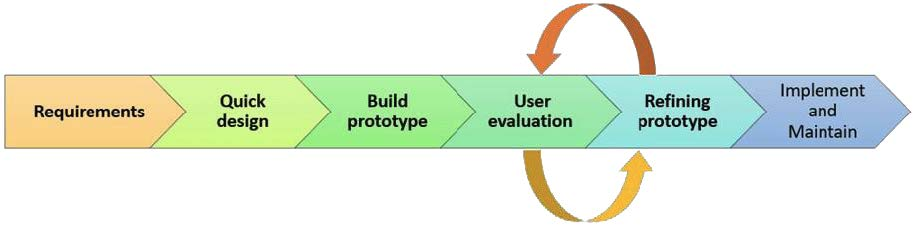
\includegraphics[]{bilder/Prototyping_Stages.jpg}
    \caption{Prototyping-Modell Stadien \cite{senarath2021waterfall}}
    \label{fig:Prototyping-Modell}
\end{figure}


Das Prototyping-Modell wurde eingesetzt, da die Anforderungen des technischen Feasibility Checks zu Beginn noch nicht eindeutig definiert waren und erst im Laufe der Entwicklung bestimmte Aspekte geklärt werden konnten. Außerdem wird das Risiko von Fehl-Entwicklungen minimiert, da der Anwender Ergebnisse schneller evaluieren kann. Zudem fördert dieses Vorgehen den regelmäßigen Austausch zwischen dem Entwickler und den Auftraggebern \cite{senarath2021waterfall}.

\section{Aufbau der Arbeit}
Die Bachelorarbeit ist so strukturiert, dass nach diesem einleitenden Kapitel in Abschnitt \ref{Chap:TheoretischeGrundlagen} die wichtigsten theoretischen Grundlagen erklärt werden. 
Hierbei wird kurz das Unternehmen Infineon Technologies AG vorgestellt und anschließend die Halbleitertechnologie behandelt. Danach wird auf die Software-Applikation \gls{REALIS} eingegangen und der technische Feasibility Check erläutert.

Im nächsten Schritt werden im Kapitel \textit{\nameref{Chap:Anforderungen}} die technischen und funktionalen Anforderungen beschrieben, die durch das Prototyping-Modell schrittweise verbessert und bei Bedarf erweitert worden sind. Zusätzlich wird eine Stakeholderanalyse durchgeführt.

Zur Realisierung der Lösung wird ein Design erstellt, das dann im Kapitel \textit{\nameref{Chap:Implementierung}} umgesetzt wird. Das Kapitel Test beschreibt die Testmethodik. Abschließend werden die während der Arbeit aufgetretenen Herausforderungen reflektiert und ein Fazit gezogen. Darüber hinaus wird ein Ausblick auf potenzielle Optimierungen und Erweiterungen des Systems bzw. Algorithmus gegeben.







	\chapter{Theoretische Grundlagen}\label{Chap:TheoretischeGrundlagen}
In diesem Abschnitt wird zunächst die Firma Infineon Technologies AG, in Kooperation mit der diese Arbeit entstanden ist, vorgestellt. Anschließend werden die theoretischen Grundlagen der Halbleitertechnologie geklärt - dem Hauptgeschäftsfeld der Infineon Technologies AG -, um den Nutzen der internen Software-Applikation \gls{REALIS} verständlich zu machen. Im darauffolgenden Kapitel, welches das System \gls{REALIS} näher bringen soll, wird auf dessen sogenannten Projekt-Lebenszyklus, die Architektur und Statistiken eingegangen. Der technische Feasibility Check, der einen spezifischen Teil dieser Applikation darstellt, wird im letzten Teil dieses Kapitels behandelt.

\section{Infineon Technologies AG}

Die Infineon Technologies AG zählt zu den weltweit führenden Herstellern von Halbleitern in den Bereichen Automotive, Power \& Sensor Systems, Green Industrial Power und Connected Secure Systems. Mit rund 58.600 Mitarbeitern ist das Unternehmen global tätig und betreibt insgesamt 84 Standorte \cite{infineon2024unternehmenspraesentation}. Einer dieser Standorte ist Regensburg mit mehr als 3000 Mitarbeitern, wo sowohl Entwicklung als auch Fertigung betrieben wird. Regensburg gilt dabei als Innovationslabor und Hightech-Fabrik, und ist der einzige Standort, an dem sowohl Frontend- als auch Backend-Produktion erfolgen. \cite{infineon2024regensburg}.

\section{Halbleitertechnologie}

Die Halbleitertechnologie ermöglicht es, elektronische Schaltungen vollständig in einem einzigen Herstellungsverfahren zu erzeugen. Dabei entstehen alle elektronischen Bauelemente und elektrischen Verbindungen auf einem monolithischen Halbleiterplättchen, das als integrierter Schaltkreis (\gls{IC}) bezeichnet wird. Diese kleinen, dünnen Plättchen bestehen in der Regel aus Silizium und werden als Chips bezeichnet. Ein fertiger Wafer ist in Abbildung \ref{fig:Silizium-Wafer} zu sehen.

Halbleitermaterialien haben die Fähigkeit, elektrischen Strom zu leiten, weisen jedoch bei Raumtemperatur einen relativ hohen Widerstand auf. Mit steigender Temperatur nimmt ihre Leitfähigkeit exponentiell zu – eine Eigenschaft, die sie von klassischen elektrischen Leitern wie Metallen unterscheidet. Die Leitfähigkeit eines Halbleiters kann durch Dotierung, das gezielte Einbringen von Fremdatomen, erheblich verändert werden.

Zur Herstellung integrierter Schaltkreise wird hochreines, monokristallines Halbleitermaterial benötigt, bei dem alle Atome in einer gleichmäßigen, durchgehenden Struktur angeordnet sind. Da solche Strukturen in der Natur nicht vorkommen, müssen sie technisch durch das „Züchten“ von Kristallblöcken in Stangenform erzeugt werden. Diese Stangen werden in dünne Scheiben, sogenannte Wafer, geschnitten, die als Ausgangsmaterial für die Chip-Produktion dienen. Ein Wafer kann je nach Größe Hunderte bis Zehntausende Chips enthalten, die alle gleichzeitig hergestellt werden können.

\begin{figure}[!h]
    \centering
    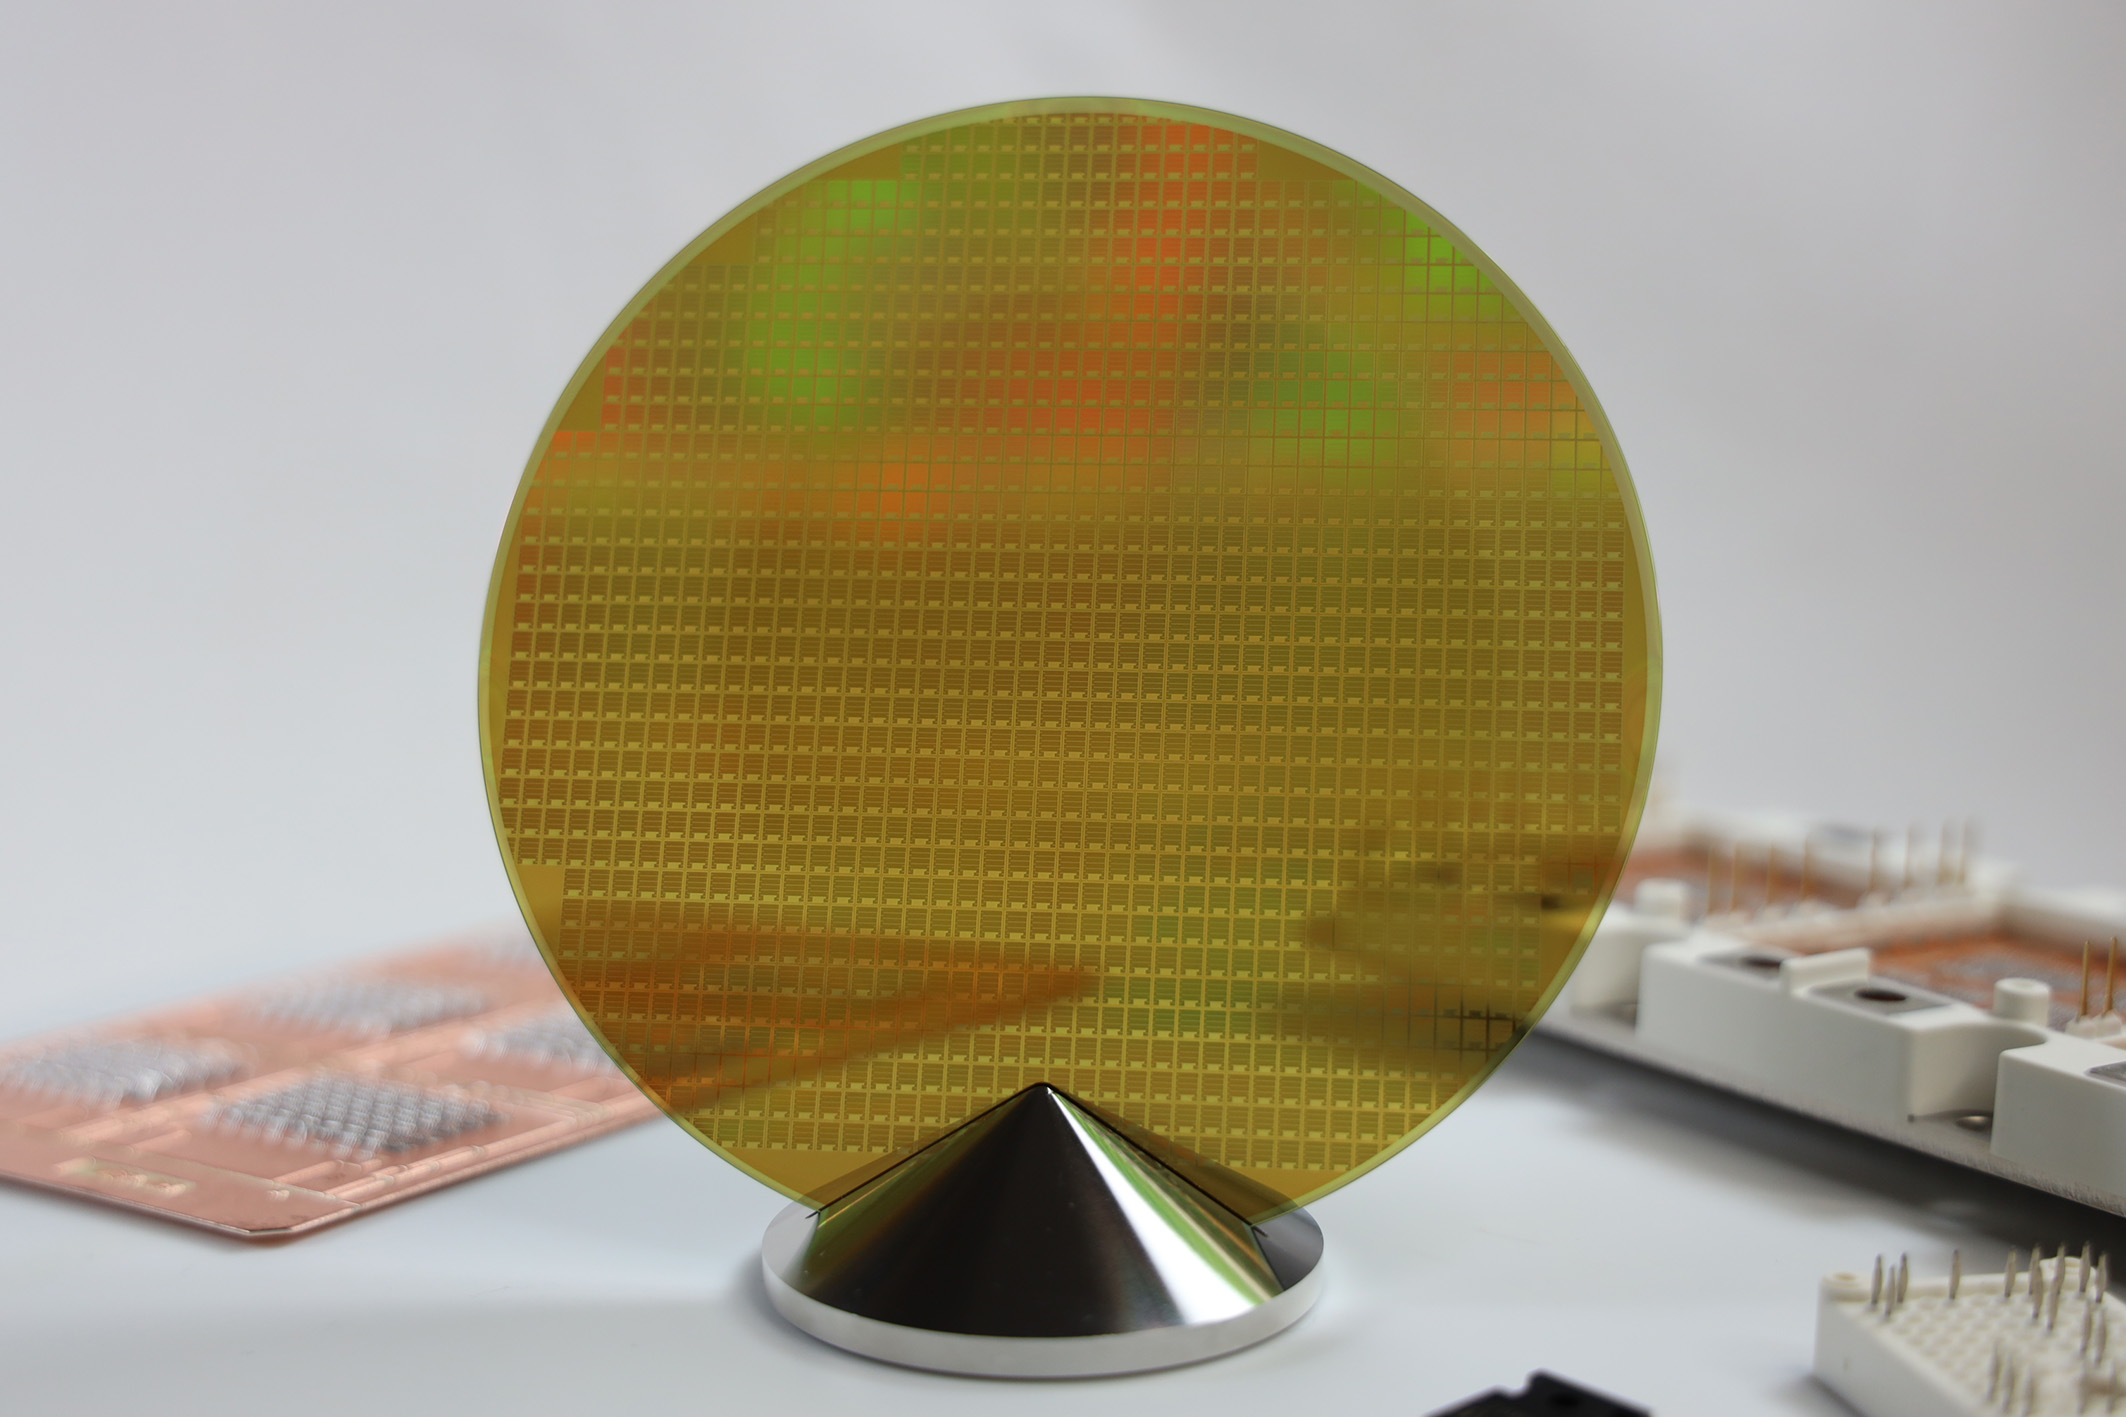
\includegraphics[width=0.9\textwidth]{bilder/SiC-Wafer-Infineon.jpg}
    \caption{Fertiger Silizium-Wafer mit Chips}
    \label{fig:Silizium-Wafer}
\end{figure}

Silizium ist das am häufigsten verwendete Material in der Halbleiterindustrie, weil es viele praktische Vorteile bietet. Es hat die perfekte Balance für den Einsatz in verschiedenen elektronischen Anwendungen und funktioniert gut bei normalen Betriebstemperaturen. Silizium bildet ein stabiles und zuverlässiges Isoliermaterial, das in Schaltkreisen vielseitig eingesetzt werden kann. Es leitet Wärme effizient ab, was wichtig ist, um eine Überhitzung zu vermeiden, besonders bei kleinen und leistungsstarken Chips. Außerdem lässt sich Silizium einfach in großen, reinen Kristallen herstellen, die für eine gleichmäßige Leistung in der Chipproduktion entscheidend sind.

Die Fertigung beginnt mit einem Rohwafer, auf dem im \gls{FEOL} alle Dotierungen erfolgen. Im darauf folgenden \gls{BEOL} werden abwechselnd isolierende und metallische Schichten aufgetragen und strukturiert, wodurch Leiterbahnen und Durchkontaktierungen entstehen. Die Strukturen moderner Chips sind dabei im Nano- bis Mikrometerbereich angesiedelt.

Am Ende des Fertigungsprozesses werden die integrierten Schaltkreise (\gls{IC}), die in parallelen Reihen und Spalten auf der Oberfläche des Wafers angeordnet sind, die in Abbildung \ref{fig:Silizium-Wafer} gut erkennbar sind, durch senkrecht verlaufende Schnitte voneinander getrennt. Durch diesen Schritt entstehen kleine, rechteckige, dünne Plättchen, die als Chips bekannt sind. Die Wafer, die aus den gezüchteten Kristallstäben mit Innenlochsägen ausgeschnitten werden, sind kreisrunde Scheiben und weisen typischerweise Dicken von knapp unter 1 mm auf. Die Durchmesser moderner Wafer liegen heute bei 200 bis 450 mm. Die Infineon Technologies AG setzt hierbei aber schon neue Maßstäbe, und hat erst vor kurzem einen Durchbruch erzielt, mit der Herstellung und Verarbeitung von Silizium-Wafern, die nur 20 Mikrometer dick sind \cite{infineon2024dünnsterWafer}.

Mit zunehmender Miniaturisierung der Halbleiterprozesse steigen die Herstellungskosten, da die Technologie komplexer wird. Jedoch sinkt durch die Verkleinerung der benötigte Platz pro Funktionseinheit auf dem Chip, was die höheren Prozesskosten kompensieren kann. Dadurch führt jede neue Chip-Generation dazu, dass mehr Leistung für den gleichen Preis erzielt wird, also eine höhere Funktionalität pro investiertem Geld \cite{lienig2023halbleitertechnologie}.
\section{REALIS}\label{Sec:REALIS}
Wird bei Infineon von einem Kunden ein neues Produkt angefordert oder entwickelt Infineon selbst ein neues Produkt, so muss dieses zunächst getestet und qualifiziert werden, bevor es in Masse produziert werden kann. Mit Produkt ist dabei ein fertiger Chip, der auf einem Wafer hergestellt wurde, gemeint. Für diese Zuverlässigkeits- bzw. Qualitäts-Tests wurde bei Infineon eine Software mit dem Namen \gls{REALIS} entwickelt. Dieses System umfasst die komplette Planung und Dokumentation der Durchführung und Ergebnisse dieser Tests. Das System beinhaltet eine gleichnamige Datenbank, in der alle wichtigen Informationen gespeichert werden.

\subsection{Projekt-Lebenszyklus}\label{Subsec:project-lifecycle}
Um ein neues Produkt zu testen, wird vom sogenannten \gls{QM} ein neues Projekt in \gls{REALIS} angelegt. Dieses befüllt er mit verschiedenen (Stress-)Tests, basierend auf vorhandenen Templates, die Arbeitsschritte (Operationen), Start- und Enddaten, Parameter der Operationen einzelner Tests und weitere Informationen enthalten. Dieser erste Schritt entspricht der obersten Zeile in Abbildung \ref{fig:realis-project-lifecycle} und bildet den Anfang eines REALIS Projekt-Lebenszyklus. 

Für jeden der folgenden Schritte wird in \gls{REALIS} der ``State``(Status) der Tests eines Projektes verändert und damit der Fortschritt dokumentiert. Dabei steht dieser zu Beginn immer auf  ``NEW`` und wird anschließend nach jedem der im Folgenden beschriebenen Schritte auf einen neuen ``State`` geändert (vgl. Abbildung \ref{fig:realis-project-lifecycle}, rechte Spalte). Welcher neue Zustand einem Test zugewiesen wird, wird dadurch entschieden, ob der beschriebene Schritt erfolgreich durchgeführt werden konnte oder nicht.

Im zweiten Schritt des Lebenszyklus weist der \gls{QM} das Projekt durch einen internen Mechanismus, einem ''State-Change'' des Projekts, einem sogenannten \gls{RPT}-Labor zu. 

In dem festgelegten \gls{RPT}-Labor validieren im Anschluss Mitarbeiter manuell die Richtigkeit der angelegten Tests und überprüfen daraufhin, ob sie die angelegten Stresstests des Projektes auch durchführen können. 
Für die Validierung der Tests werden die Stressparameter auf deren Sinnhaftigkeit überprüft. Die Frage der Durchführbarkeit hängt davon ab, ob im zugewiesenen \gls{RPT}-Labor Maschinen vorhanden sind, die in der Lage sind, die geforderten Stressoperationen auszuführen und die festgelegten Stressparameter einzuhalten. Zudem müssen diese Maschinen verfügbar sein – also weder in Benutzung noch außer Betrieb.

Diese Prüfungen bezeichnen den aktuellen technischen Feasibility Check, dessen Ergebnisse in \gls{REALIS} dokumentiert werden.
Falls für einige Operationen bzw. Tests keine gültigen Maschinen vorhanden sind, werden diese Tests an andere \gls{RPT}-Labore delegiert. Dadurch müssen die zu testenden Produkte jedoch von einem Labor zum anderen transportiert werden, was aufgrund der weltweiten Verteilung viel Zeit in Anspruch nehmen kann.

\begin{figure}[!h]
    \centering
    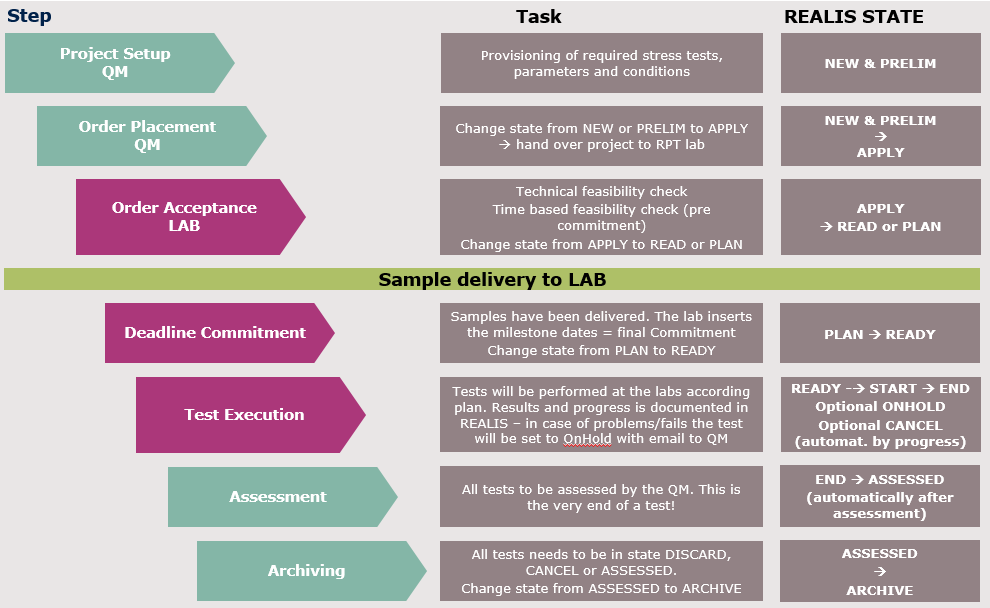
\includegraphics[width=1\textwidth]{bilder/realis-project-lifecycle.png}
    \caption{REALIS Projekt-Lebenszyklus \cite{REALISWikiIntern}}
    \label{fig:realis-project-lifecycle}
\end{figure}

Anschließend wird ein ''Sample'', also eine kleine Stückzahl des Produktes, zum beauftragten \gls{RPT}-Labor geschickt. Das ''Sample'' wird in der Fachsprache auch als \textit{Test lot}, oder zu Deutsch: \textit{Test-Los} bzw. nur \gls{los} bezeichnet. Die Stückzahl wird dabei in \gls{REALIS} dokumentiert. Die  Daten der Testoperation werden dann final festgelegt und der Test-Status wird geändert.

Daraufhin erfolgt die planmäßige Durchführung der einzelnen Operationen der\linebreak Stresstests. Dabei werden der Fortschritt und die Ergebnisse von Labor-Mitarbeitern, sogenannten \glspl{operator}, in \gls{REALIS} dokumentiert. Treten während der Stresstests Probleme oder Fehler auf, werden diese an den \gls{QM} weitergeleitet, der über das weitere Vorgehen entscheidet.

Nachdem alle Tests vollständig durchgeführt und dokumentiert worden sind, muss der \gls{QM} die Ergebnisse prüfen und bewerten. Zum Schluss werden die Tests dann archiviert, wobei aus Gewährleistungsgründen die Chips und Testergebnisse 16 Jahre aufbewahrt werden müssen. Damit ist der Projekt-Lebenszyklus abgeschlossen.

\subsection{Architektur und Technologie}
Das ursprüngliche Frontend von REALIS war eine Windows-Desktop-Applikation, die sowohl vom \gls{RPT}-Labor-Mitarbeiter als auch vom \gls{QM} genutzt wurde. Im Zuge einer Modernisierung wird das System schrittweise zu einer Web-Applikation migriert. Zeitgleich erfolgt eine Aufteilung in zwei separate Anwendungen, eine für den \gls{QM} und eine für den \gls{operator}, mit dem Ziel, die Geschäftsprozesse zu vereinfachen und die Nutzerfreundlichkeit zu verbessern.

Abbildung \ref{fig:realis-komponentendiagramm} zeigt die aktuelle Systemarchitektur in Form eines Komponentendiagramms. Im Backend (grün dargestellt) kommuniziert der \texttt{REALIS-Server} über eine \texttt{DataAccess}-Schnittstelle direkt mit der zentralen \texttt{REALIS-Datenbank}, welche auf Oracle basiert. Der \texttt{REALIS-Server} stellt die Geschäftslogik (Business-Layer) bereit und wird über eine \texttt{REST-API} von den Frontends genutzt.

\begin{figure}[!h]
    \centering
    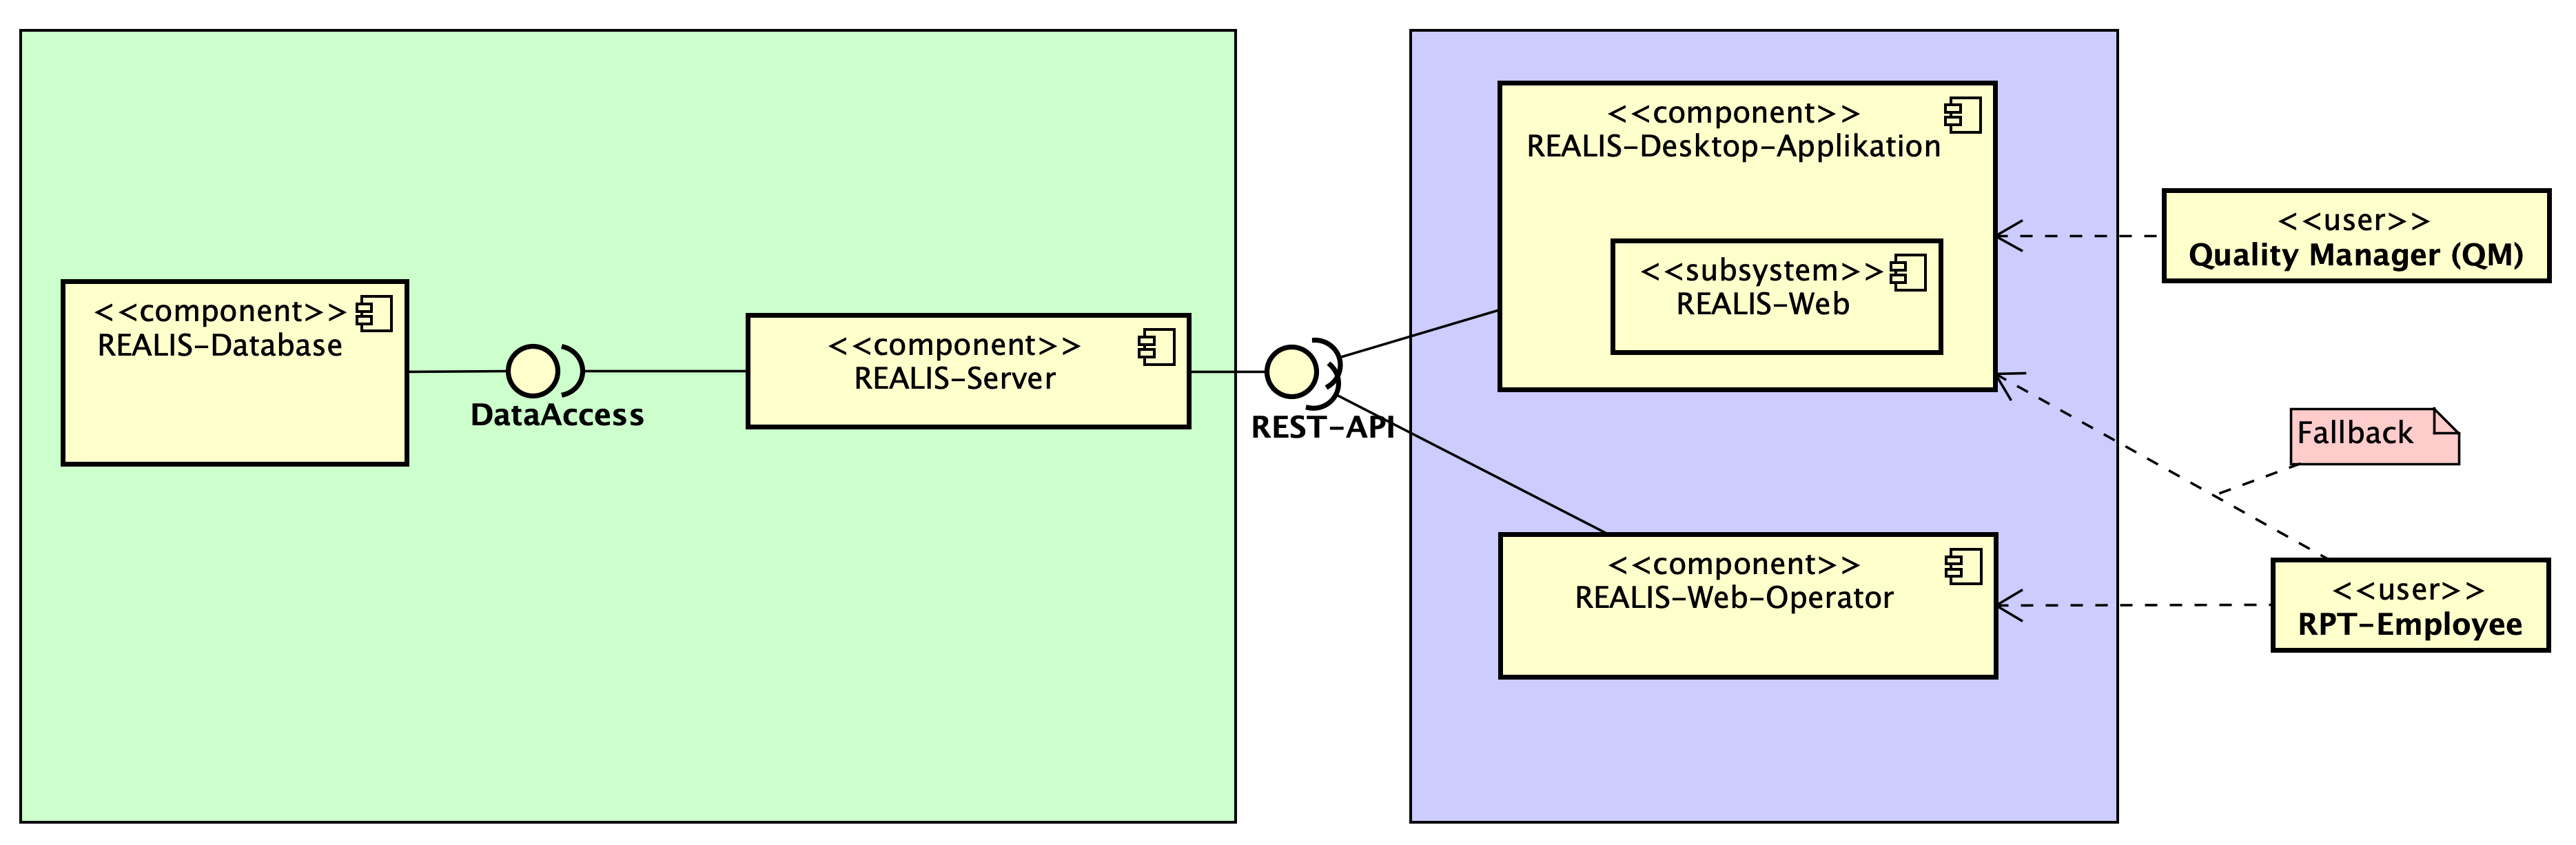
\includegraphics[width=1\textwidth]{bilder/REALIS-Komponentendiagramm2.png}
    \caption{REALIS Komponentendiagramm}
    \label{fig:realis-komponentendiagramm}
\end{figure}

Das Frontend besteht aus zwei Hauptkomponenten (blau dargestellt):
\begin{enumerate}
    \item \textbf{REALIS-Desktop-Applikation:} \\
Die ursprüngliche Desktop-Anwendung, die sukzessive durch die Integration von neuen Web-Funktionalitäten modernisiert wird.\\
Diese Web-Module, die mit dem Framework Angular entwickelt werden, sind als Subsystem (\texttt{REALIS-Web}) innerhalb der Desktop-Applikation eingebettet. Dieses System steht sowohl dem \gls{QM} als auch dem \gls{RPT}-Labor-Mitarbeiter zur Verfügung.

\item \textbf{REALIS-Web-Operator-System:} \\
Eine eigenständige Web-Applikation, die speziell für die Anforderungen des \gls{RPT}-Labors konzipiert wird. \\
Diese Anwendung befindet sich noch in der Entwicklung, wird jedoch bereits für einige Aufgaben eingesetzt. Für nicht implementierte Funktionen muss der \gls{RPT}-Mitarbeiter vorübergehend auf die alte Desktop-Applikation ausweichen. Zusätzlich ist geplant, das \texttt{REALIS-Web-Operator-System} als native iOS-App für mobile Apple-Geräte (z. B. iPads, iPhones) bereitzustellen. Die Verwendung des Angular Frameworks ermöglicht dabei eine plattformübergreifende Programmierung, die sowohl als Web-App als auch als native App funktioniert.
\end{enumerate}

Das Diagramm \ref{fig:realis-komponentendiagramm} verdeutlicht die Trennung zwischen Backend und Frontend sowie die unterschiedlichen Nutzerrollen (\gls{QM} und \gls{RPT}-Employee), die spezifische Zugriffsrechte auf die jeweiligen Systeme haben.


\subsection{Weitere Funktionen und Statistiken}
Neben der Möglichkeit Qualitätstests (Reliability-Tests) anzulegen, bietet \gls{REALIS} eine Vielzahl zusätzlicher Funktionen, die dazu beitragen, Prozesse effizienter zu gestalten und Engpässe zu vermeiden. So unterstützt das System beispielsweise bei der Planung individueller Laborkapazitäten, wodurch unnötige Investitionen vermieden und vorhandene Ressourcen optimal genutzt werden können. Darüber hinaus ermöglicht \gls{REALIS} die Referenzierung bereits durchgeführter Testergebnisse, um redundante Tests zu vermeiden und Zeit sowie Kosten zu sparen.

Nach Abschluss eines Tests können in \gls{REALIS} automatisch benötigte Ergebnisberichte generiert werden – sowohl für den Kunden als auch für das \gls{RPT}-Labor. Dies erleichtert die Dokumentation und erhöht die Effizienz im Testmanagement.

Seit 2001 ist \gls{REALIS} im Einsatz und verzeichnet derzeit etwa 4.300 aktive Nutzer. Das System findet Anwendung in 101 \gls{RPT}-Laboren in 17 Ländern. Aktuell verwaltet \gls{REALIS} rund 270.000 Projekte mit etwa 1,9 Millionen Stresstests \cite{REALISPowerPointIntern}.
\section{Technischer Feasibility Check}
Der automatisierte technische Feasibility Check, bezeichnet eine ''Machbarkeitsprüfung'', die bewertet, ob ein Stresstest an einem \ac{RPT}-Laborstandort durchgeführt werden kann.

Dieser Check ist ein integraler Bestandteil des \ac{REALIS}-Projekt-Lifecycles, wie in Kapitel \ref{Subsec:project-lifecycle} beschrieben. Derzeit wird er manuell von Mitarbeitern des \ac{RPT}-Labors durchgeführt. Dabei tragen sie in der Software-Applikation \ac{REALIS} in einem einfachen Feld ''Yes'' oder ''No'' ein, um die Durchführbarkeit zu bestätigen. Zuvor prüfen sie, ob die im Labor vorhandenen Kapazitäten und Bedingungen ausreichen, um die geforderten Tests für das jeweilige Produkt durchzuführen.

Die Beurteilung basiert auf mehreren Parametern. Um diese besser zu verstehen, wird im folgenden Kapitel erläutert, wie ein Stresstest im Detail abläuft und welche Schritte dabei erforderlich sind.


\subsection{Stresstests (Reliability Tests)}

Stresstests, auch als \textit{Reliability Tests} bezeichnet, dienen der Qualifikation eines neuen Produkts und umfassen verschiedene Testarten. Zu den gängigsten gehören Temperaturtests (Hitze- und Kältetests), Drucktests, Feuchtigkeitstests sowie elektrische Tests. Oder auch Kombinationen dieser Testarten.

Jeder Stresstest setzt sich aus mehreren aufeinanderfolgenden Operationen zusammen, die von einem \ac{RPT}-Labor-\gls{operator} mithilfe eines Test-Lots (einer kleinen Stückzahl des Produkts) durchgeführt werden. Typischerweise beginnt ein Test mit einer ''START''-Operation und endet mit einer ''END''-Operation. Dazwischen befinden sich mehrere Stressoperationen, die den jeweiligen Stresstypen des Tests widerspiegeln und die eigentliche Belastungsprüfung darstellen.

Zwischen den Stressoperationen werden Funktionsprüfungen durchgeführt, bei denen der \gls{operator} alle Teile des Test-Lots auf ihre Funktionalität überprüft. So wird sichergestellt, dass das Produkt die vorhergehende Stressoperation unbeschadet überstanden hat.

Darüber hinaus gibt es sogenannte Transfer-Operationen. Diese sind erforderlich, wenn Produkte während eines Tests zwischen verschiedenen \ac{RPT}-Laboren transportiert werden müssen.

	\chapter{Anforderungen}\label{Chap:Anforderungen}

In diesem Kapitel werden die Anforderungen an den technischen Feasibility Check strukturiert dargestellt. Dabei werden die funktionalen Anforderungen durch nicht-funktionale Anforderungen ergänzt, die Aspekte wie \todo{was umfassen}Performance, Benutzerfreundlichkeit und Sicherheit umfassen.

Anschließend wird eine Stakeholderanalyse durchgeführt, um die beteiligten Personengruppen am Projekt zu identifizieren, und deren Interessen Bedürfnisse und Einflüsse zu verstehen. 

\section{Funktionale Anforderungen} \label{Sec:funktionale-anforderungen}

\setlength{\leftskip}{1em} 
\textbf{Automatisierung des technischen Feasibility Checks}  \\
Der technische Feasibility Check soll vollständig automatisiert erfolgen, sodass keine technischen Vorkenntnisse seitens der Benutzer erforderlich sind. Die Ausführung wird ausschließlich durch den Benutzer initiiert oder angefordert. Durch die Automatisierung sollen menschliche Fehler reduziert, und die Genauigkeit der Entscheidungen deutlich gesteigert werden.

\textbf{Nachvollziehbarkeit}  \\
Um die Ergebnisse des automatisierten Feasibility Checks transparent und nachvollziehbar zu machen, müssen alle zugrunde liegenden logischen Entscheidungen in verständlicher Form für den Benutzer aufbereitet werden. Dies ist besonders wichtig, wenn die Logik auf unerwartete Probleme stößt. Darüber hinaus ermöglicht die Automatisierung eine fundierte Begründung der Entscheidungen, die über die bisherige einfache „Ja/Nein“-Auswahl hinausgeht.

\textbf{Modularer Aufbau}  \\
Der Feasibility Check besteht aus mehreren separaten ''Checks'' (wie Condition und Equipment Check). Diese Module, abhängig von den Parametern (siehe Kapitel~\ref{Subsec:ParameterdestechnischenFeasibilityChecks}), sollen von Systemadministratoren individuell aktiviert oder deaktiviert werden können. Ist ein Modul deaktiviert, soll der Benutzer weiterhin die Möglichkeit haben, den Check manuell durchzuführen.

\textbf{Flexibilität und Erweiterbarkeit}  \\
Das System soll so konzipiert sein, dass neue Module bzw. ''Checks'' flexibel hinzugefügt werden können, um zukünftige Anforderungen ohne größeren Aufwand zu erfüllen.

\textbf{Manuelle Durchführung weiterhin Ermöglichen}  \\
Falls der automatisierte Feasibility Check zu einem negativen Ergebnis kommt, auch aufgrund von Problemen in der bestehenden Logik, soll der Benutzer die Möglichkeit haben, den Check manuell durchzuführen.

\textbf{Integration in bestehende Architektur}  \\
Die Systemarchitektur des Feasibility Checks muss vollständig kompatibel mit der bestehenden Architektur von \gls{REALIS} sein, um eine nahtlose Integration zu gewährleisten.

\setlength{\leftskip}{0em} 

\section{Nicht-funktionale Anforderungen}

\setlength{\leftskip}{1em} 
\textbf{Persistenz}  \\
Ergebnisse und logische Entscheidungen des Feasibility Checks müssen dauerhaft und eindeutig mit dem zugehörigen Stresstest in der Datenbank gespeichert werden.

\textbf{Datenintegrität}  \\
Während der Ausführung eines Feasibility Checks darf kein anderer Benutzer oder Systemprozess Änderungen an dem betreffenden Test vornehmen können.

\textbf{Test- und Rollout-Strategie}  \\
Der Feasibility Check soll zuerst in einer Testumgebung eingeführt und gründlich getestet werden. Nach erfolgreicher Validierung erfolgt der Rollout auf die produktive Umgebung.

\textbf{Fehlerrobustheit}  \\
Der Feasibility Check muss bei unerwarteten Situationen (z. B. unvollständige Parameter, Dateninkonsistenzen) mit klar definierten Fehlermeldungen reagieren und dabei stabil bleiben.

\textbf{Unittests und Wartung}  \\
Um sicherzustellen, dass der Feasibility Check auch bei zukünftigen Systemänderungen wie erwartet funktioniert, müssen umfassende Unittests implementiert werden.

\textbf{Performance}  \\
Obwohl keine festen Zeitvorgaben bestehen, soll der Feasibility Check ressourcenschonend im Hintergrund ablaufen, um die Benutzerfreundlichkeit zu erhöhen.

\textbf{Codequalität und Dokumentation}  \\
Der Quellcode des Feasibility Checks muss klar strukturiert und umfassend dokumentiert sein. Ziel ist es, die Logik für andere Entwickler leicht verständlich zu machen und zukünftige Änderungen oder Erweiterungen zu erleichtern.


\setlength{\leftskip}{0em} % Rückstellung

\section{Stakeholder-Analyse}
Im Rahmen der Entwicklung des automatisierten technischen Feasibility Checks erfolgte mehrfach wöchentlich ein Austausch mit den Stakeholdern. Diese setzen sich aus vier Schlüsselpersonen sowie einem Entwicklungsteam zusammen.

Zu den Schlüsselpersonen gehören der Product Owner von \gls{REALIS}, der Application Owner, der Scrum Master sowie ein LabAdmin des \gls{RPT}-Labors in Regensburg. Ergänzt wird diese Gruppe durch das Infineon externe Entwicklungsteam von \gls{REALIS}, dessen Mitglieder in Portugal ansässig sind.

Der \textbf{Product Owner} von \gls{REALIS} fungiert als Interessenvertreter der Stakeholder, zu denen die \gls{RPT}-Labore und \glspl{QM} zählen, mit dem Bestreben, ein konsentiertes Produktziel zu entwickeln. Seine Hauptaufgabe besteht darin, die Anforderungen zu priorisieren und in klar formulierte Einträge im Product Backlog für das Entwicklungsteam zu überführen. Dabei stellt er sicher, dass das Team kontinuierlich an den wichtigsten Aufgaben arbeitet \cite{scrumguide2020}.

Der \textbf{Application Owner} trägt die Verantwortung für die strategische Ausrichtung und die langfristige Verwaltung von \gls{REALIS}. In seiner Rolle als Applikations-Architekt sorgt er für die Einhaltung der Architektur-Richtlinien. Zu seinen Aufgaben gehören die kontinuierliche Optimierung der Anwendung, die Gewährleistung ihrer Stabilität und Sicherheit sowie die Planung von Systemaktualisierungen, wie etwa dem Wechsel vom Desktop-Frontend zu einer webbasierten Anwendung, um den geschäftlichen Anforderungen gerecht zu werden.

Der \textbf{Scrum Master} moderiert die agilen Prozesse und achtet darauf, dass diese korrekt eingehalten werden. Er unterstützt das Team dabei, sich kontinuierlich zu verbessern und effizienter zu arbeiten. Zudem fördert er die Zusammenarbeit zwischen den Teammitgliedern und schafft ein produktives Arbeitsumfeld. Hierfür beseitigt er Hindernisse zwischen den Stakeholdern und dem Scrum Team \cite{scrumguide2020}.

Der \textbf{LabAdmin} im \gls{RPT}-Labor in Regensburg assistiert den \gls{RPT}-Labor-\glspl{operator} bei ihrer Tätigkeit und hilft bei der Lösung von Problemen im Umgang mit \gls{REALIS}. Da\-rüber hinaus entwickelt er Projekt-Test-Templates in \gls{REALIS}, die \glspl{QM} beim Anlegen von Tests in Projekten unterstützen. Er ist zudem aktiv in das Testen neuer Software-Versionen von \gls{REALIS} eingebunden.


Das \textbf{externe Entwicklungsteam} von \gls{REALIS} mit Sitz in Portugal stellt sicher, dass die Coding-Standards eingehalten werden. Es legt besonderen Wert auf eine stabile und gut dokumentierte Programmierung, um die Wartbarkeit und Weiterentwicklung des Codes zu gewährleisten.






	\chapter{Systemarchitektur}

\section{Architekturüberblick}
Gesamtsicht auf die Architektur der Lösung (Backend, Frontend, Datenbank).

\begin{figure}[!h]
    \centering
    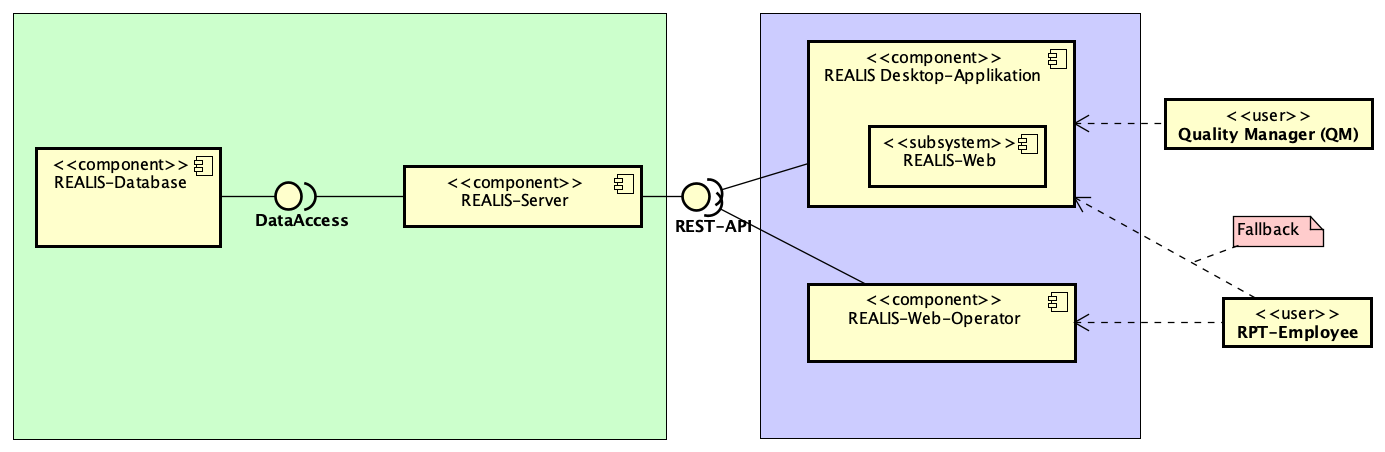
\includegraphics[width=1\textwidth]{bilder/REALIS-Komponentendiagramm.png}
    \caption{REALIS Komponentendiagramm}
    \label{fig:realis-komponentendiagramm}
\end{figure}

\section{Datenbankdesign}
Struktur der Oracle-Datenbank, wichtige Tabellen und Beziehungen.

\section{Backend-Logik}
Beschreibung der C\#-Implementierung, inklusive wichtiger Klassen und Methoden.

\section{Frontend-Design}
Überblick über die Angular-Anwendung, Struktur und Benutzeroberfläche.

	\chapter{Implementierung}\label{Chap:Implementierung}

\section{Projektplan für den Feasibility Check}\todo{Kapitel am anfang von Systemdesign tun}
Für die Entwicklung des automatisierten technischen Feasibility Checks wurde zu Beginn ein Projektplan in Form eines GANTT-Diagramms erstellt, der in Abbildung \ref{fig:roadmap} dargestellt ist. Dieser Plan ist in mehrere Swimlanes unterteilt und umfasst die Erarbeitung der Anforderungen, den Entwurf des Datenbankdesigns, die Backend-Entwicklung, die Frontend-Entwicklung sowie das Testen des Systems. Zusätzlich wurden für die Benutzer spezifische Meilensteine definiert, die in der unteren Zeile des Diagramms veranschaulicht werden.

\begin{figure}[!htbp]
    \centering
    \includegraphics[width=1\textwidth]{bilder/Roadmap.pdf}
    \caption{Feasibility Check Projektplan}
    \label{fig:roadmap}
\end{figure}

Die geplanten Maßnahmen für die ersten zwei Monate konnten weitgehend umgesetzt werden, mit Ausnahme der Endanwender-Tests. In den darauffolgenden Monaten lag der Schwerpunkt auf der Überarbeitung bestehender Algorithmen im Backend, da wiederholt neue Ausnahmefälle identifiziert wurden. Auch das Frontend wurde mehrfach angepasst, um den aktuellen Anforderungen gerecht zu werden. Dadurch konnten alle optionale Meilensteine, sowie die Implementierung weiterer Checks inklusive des er \gls{substrate} Checks, nicht realisiert werden – unter anderem aufgrund einer zu optimistischen Zeiteinteilung.

Aktuell sind das Datenbankdesign und das Backend bereits vom Testing-System auf das Staging-System ausgerollt worden und werden dort von einzelnen Anwendern getestet. Für das Backend wurden zudem Unittests entwickelt, was im Frontend leider nicht mehr möglich war. Weitere geplante Meilensteine konnten letztlich aufgrund von Zeitbeschränkungen nicht umgesetzt werden.


\section{Entwicklungsumgebung}
Tools und Technologien, die verwendet wurden (IDE, Frameworks, Datenbank-Tools).
Angular, Visual Studio Code, 
C\#, Visual Studio,
Oracle, Pl sql developer

\section{Implementierung des Feasibility Checks}
Detaillierte Beschreibung des Implementierungsprozesses.
(Beschreibung der C\#-Implementierung, inklusive wichtiger Klassen und Methoden.
flussdiagramme
nhibernate, try catch blöcke,)
\section{Integration}
Wie die verschiedenen Teile (Frontend, Backend, Datenbank) miteinander interagieren.

\begin{figure}[!h]
    \centering
    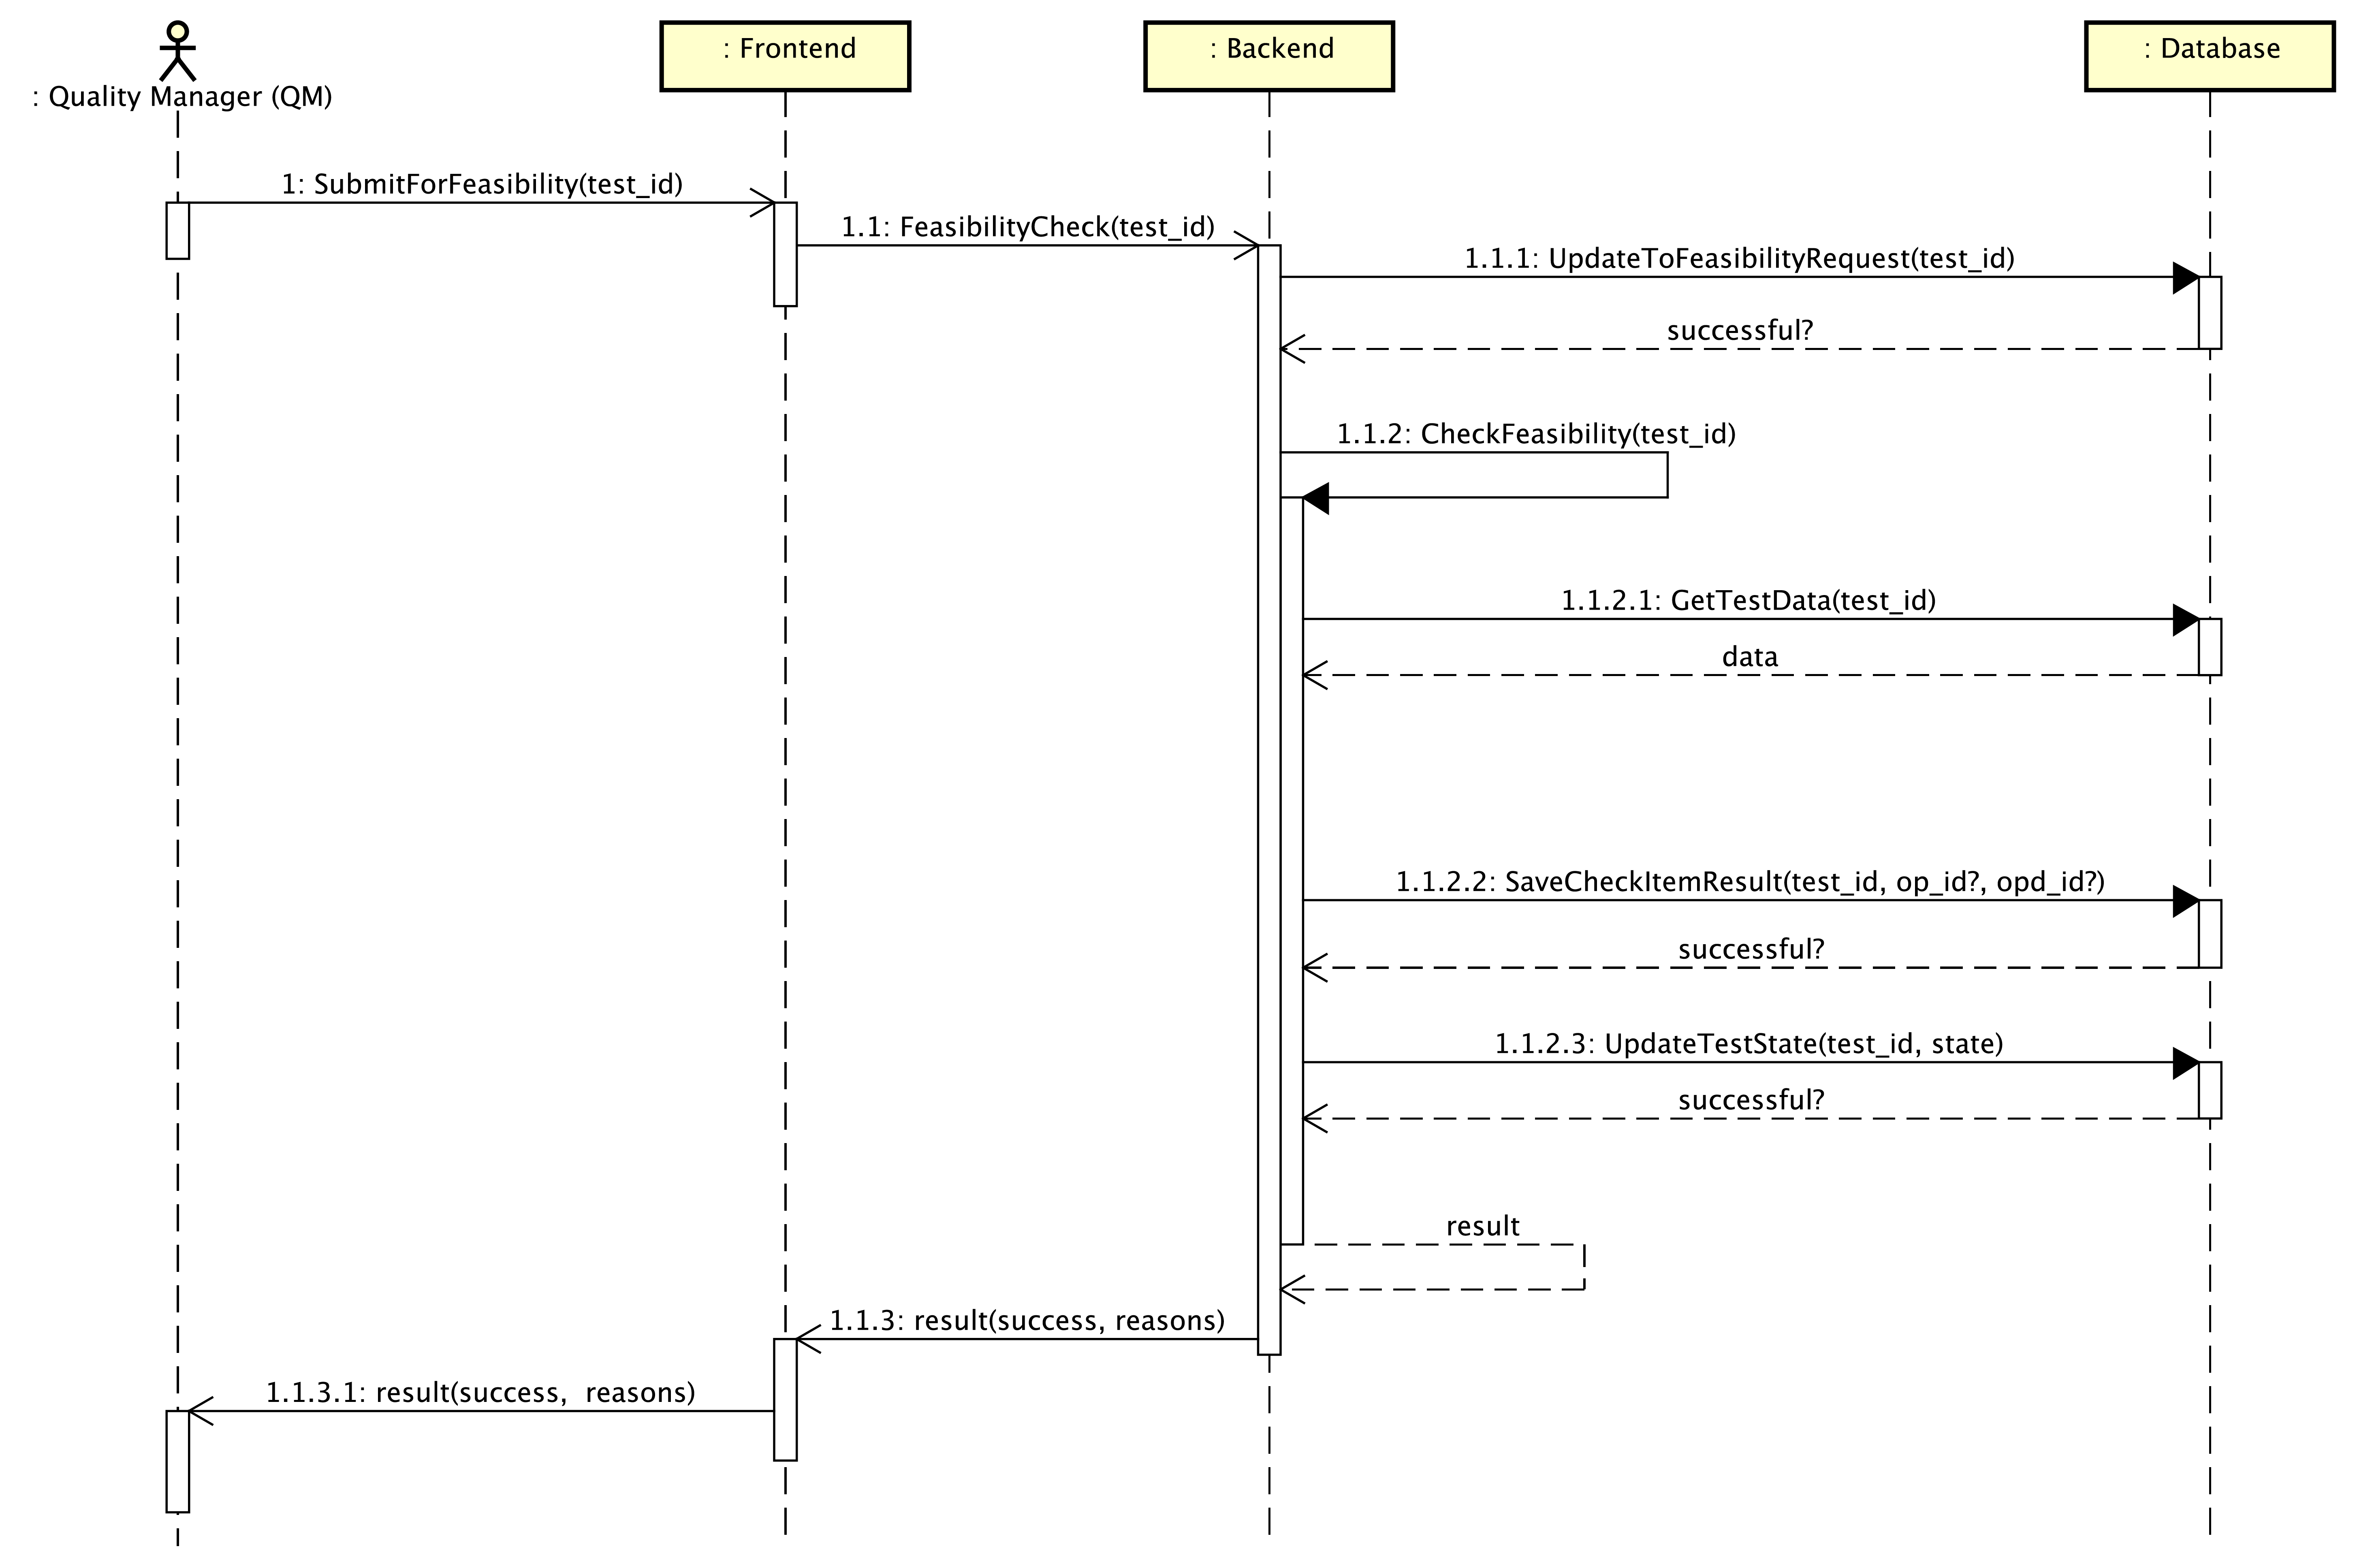
\includegraphics[width=1\textwidth]{bilder/Sequence-Integration.png}
    \caption{Sequenz-Diagramm FeasibilityCheck}
    \label{fig:sequence-diagram}
\end{figure}

	\chapter{Test und Evaluation}

Bisher ist der Feasibility Check erst in geringem Umfang von tatsächlichen Endanwendern genutzt worden; sämtliche bisher durchgeführten Tests beziehen sich bislang auf Unittests der Backend-Logik. Diese wurden jedoch mit großem Aufwand und hoher Sorgfalt entwickelt, um die langfristige Stabilität der bestehenden Logik zu gewährleisten und Regressionen bei zukünftigen Änderungen zu vermeiden.

\section{Unittests}

Die Entwicklung der Unittests für den Feasibility Check gestaltete sich als besonders anspruchsvoll. Anders als bei typischen Unittests reicht eine reine Übergabe fehlerhafter Eingaben an die Methode \texttt{FeasibilityCheck()} nicht aus, um deren Funktionalität umfassend zu testen. Stattdessen ist es sinnvoller der Methode eine valide Test-ID zu übergeben, die auf in der Datenbank gespeicherten Operationen und Parameter referenziert. Darüber hinaus hängt das Ergebnis des Feasibility Checks von mehreren Faktoren ab, wie etwa der Feasibility-Konfiguration, den einzelnen Condition- und Equipment-Checks, der \texttt{op\_data\_param\_type}-Tabelle sowie den in der Datenbank vorhandenen Maschinen.

Aufgrund dieser Komplexität ist es notwendig, gezielt ''Dummy-Daten'' in der Datenbank anzulegen. Auf Basis dieser Testdaten wird der Feasibility Check ausgeführt und das Ergebnis auf Korrektheit und Vollständigkeit validiert. Nach erfolgreicher Überprüfung erfolgt eine sichere Entfernung der ''Dummy-Daten'', um die Integrität der Datenbank zu gewährleisten.

Um diesen Prozess zu vereinfachen, dient als strukturelle Grundlage die eigens entwickelte Klasse \texttt{FeasibilityCheckScenario}, welche auf der \texttt{ProjektScenario}-Klasse aufbaut. Während letztere das Anlegen von Projekten in der REALIS-Datenbank vereinfacht, erweitert die \texttt{FeasibilityCheckScenario}-Klasse diese Funktionalität um einen Satz konfigurierbarer Methoden zur effizienten Testfallgenerierung für den Feasibility Check. Über Boolean-Parameter können gezielt Szenarien aktiviert werden, die interne ''Dummy-Daten'' erzeugen (siehe Abbildung~\ref{fig:unittests-parameters}). Beispielsweise simuliert der Boolean-Parameter \texttt{PlanValueOutOfRange} die Überschreitung zulässiger Parameterbereiche, während \texttt{WrongMachineDate} eine Datumsinkonsistenz bei Maschinendaten provoziert.

Standardmäßig sind alle Szenarien deaktiviert und können je nach Bedarf einzeln oder in Kombination aktiviert werden. Abbildung~\ref{fig:unittests-parameters} veranschaulicht die möglichen Boolean-Parameter, die als Szenarien innerhalb der \texttt{FeasibilityCheckScenario}-Klasse dienen.

\begin{figure}[!htb]
    \centering
    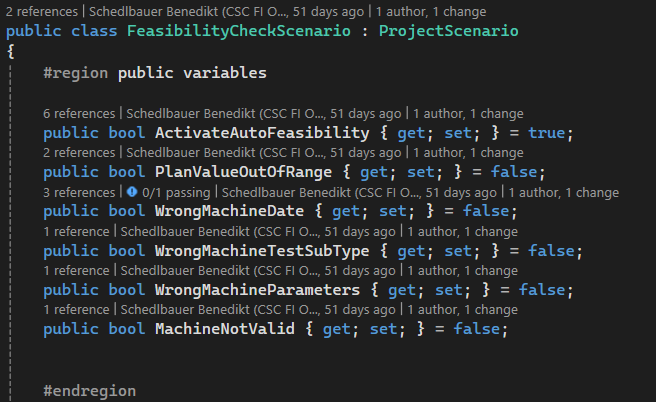
\includegraphics[width=1\textwidth]{bilder/unittests-parameters.png}
    \caption{Boolean-Parameter der \texttt{FeasibilityCheckScenario}-Klasse}
    \label{fig:unittests-parameters}
\end{figure}

Durch diese abstrahierte Vorgehensweise lassen sich die umfangreichen Unittests strukturiert und effizient umsetzen. Zwei Beispiel-Unittests sind in Abbildung~\ref{fig:unittestcases} dargestellt. Hierbei legt die Methode \texttt{CreateDefaultFeasibilityProject()} einen Default-Test an, der jeweils mit nur einer Operation und einem Parameter befüllt wird, um das Testszenario zu vereinfachen. Anschließend generiert die Methode \texttt{CreateMockData()} in der Datenbank alle erforderlichen ''Dummy-Daten'' bzw. passt bestehende Datensätze an, beispielsweise in der Feasibility-Konfigurationstabelle. Die Erstellung dieser ''Dummy-Daten'' erfolgt abhängig von den eingestellten \linebreak Boolean-Parametern, sodass die entsprechenden Szenarien erfüllt werden. Im zweiten Unittest, wie in Abbildung~\ref{fig:unittestcases} gezeigt, wurde beispielsweise das Szenario \texttt{WrongMachineDate} aktiviert. Danach wird über die Methode \texttt{PerformFeasibilityCheck()} der Feasibility Check ausgeführt, wobei das zurückgelieferte Ergebnis abschließend evaluiert wird. Ein automatisierter ''Cleanup-Mechanismus'' sorgt schließlich dafür, dass die initial angelegten ''Dummy-Daten'' sicher wieder aus der Datenbank entfernt werden.

\begin{figure}[!htb]
    \centering
    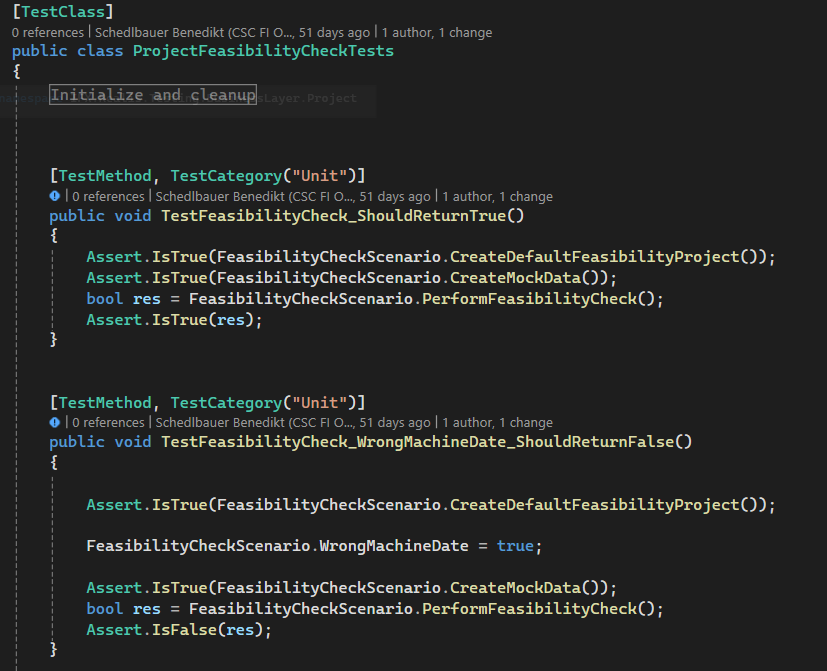
\includegraphics[width=1\textwidth]{bilder/unittestcases.png}
    \caption{Unittests für den Feasibility Check}
    \label{fig:unittestcases}
\end{figure}

Die Unittests sind in ein automatisiertes Test-Framework integriert, sodass bei jeder Änderung der Backend-Logik automatisch überprüft wird, ob alle Testfälle weiterhin erfolgreich durchlaufen werden. Diese Vorgehensweise unterstützt die kontinuierliche Qualitätssicherung und trägt maßgeblich zur Stabilität und Wartbarkeit des Systems bei.

\section{Ergebnisse der Tests}

Die umfangreichen Unittests haben wertvolle Einblicke in die Funktionsweise und Stabilität des Feasibility Checks geliefert. Die zentralen Erkenntnisse lassen sich wie folgt zusammenfassen:

\begin{itemize}
    \item \textbf{Standard-Szenario:} Bei korrekter Konfiguration und gültigen Eingabedaten wird der Feasibility Check ohne Fehlermeldungen abgeschlossen. Dies zeigt, dass die Standardlogik robust implementiert ist.
    \item \textbf{Spezifische Fehlerszenarien:} Durch die Aktivierung von Szenarien wie \texttt{PlanValueOutOfRange} und \texttt{WrongMachineDate} konnten gezielt Fehlerfälle simuliert werden. Die Tests bestätigten, dass diese Situationen korrekt erkannt und mit den vorgesehenen Fehlermeldungen quittiert werden.
    \item \textbf{Wiederholbarkeit:} Alle Testfälle lieferten bei wiederholter Durchführung konsistente Ergebnisse, was die Zuverlässigkeit der Testumgebung bestätigt.
\end{itemize}


\section{Evaluation des Systems}

Die Evaluation des Gesamtsystems stellt einen zentralen Bestandteil der Qualitätssicherung dar. Bislang lag der Fokus der Tests primär auf den Backend-Komponenten, wodurch indirekt auch die Datenbank validiert wurde. Die \texttt{FeasibilityCheckScenario}-Klasse bietet hierbei eine fundierte Basis für die zukünftige Implementierung spezifischer Anwendungsfalltests. Das Frontend wurde jedoch noch nicht in die Testprozesse einbezogen.

Um eine vollständige Validierung des Systems – bestehend aus Frontend, Backend und Datenbank – zu gewährleisten, ist die Entwicklung gezielter Unittests für das Frontend unerlässlich. Nur durch eine systematische Überprüfung aller Komponenten kann sichergestellt werden, dass diese fehlerfrei funktionieren und nahtlos miteinander interagieren.

Zusätzlich ist eine praxisorientierte Evaluation durch Endanwender von entscheidender Bedeutung. Durch Tests in realen Nutzungsszenarien können potenzielle Schwachstellen identifiziert und behoben werden. Ein iterativer Testprozess, der sowohl automatisierte als auch manuelle Tests integriert, gewährleistet, dass das System den Anforderungen des produktiven Einsatzes entspricht und kontinuierlich optimiert werden kann.


	\chapter{Diskussion}
In diesem Kapitel werden die zentralen Aspekte der Systementwicklung reflektiert und diskutiert. Dabei werden die Herausforderungen, die während des Projekts aufgetreten sind, analysiert und ein Ausblick auf mögliche Weiterentwicklungen und Optimierungen des Systems gegeben, um dessen zukünftige Einsatzfähigkeit und Effizienz zu steigern. Die Diskussion dient dazu, die gemachten Erfahrungen zu strukturieren und Potenziale für zukünftige Arbeiten aufzuzeigen.
\section{Herausforderungen}

Eine erste Herausforderung und zentrale Aufgabe war die Ausarbeitung der Anforderungen (Requirements). Dies erforderte eine präzise Kommunikation mit den Stakeholdern, um sicherzustellen, dass alle funktionalen und nicht-funktionalen Anforderungen eindeutig definiert und umfassend dokumentiert werden. 

Schwierig war zudem, sich in das umfangreiche und komplexe Datenbankmodell von \gls{REALIS} einzuarbeiten. Die Größe und Komplexität des Modells machten es notwendig, sich intensiv mit der Struktur und den Zusammenhängen der Daten auseinanderzusetzen, um die für den Feasibility Check relevanten Tabellen zu identifizieren. Nur durch dieses tiefgehende Verständnis konnte garantiert werden, dass die Erweiterungen effizient und korrekt in das System integriert werden konnten.

Zu den Herausforderungen zählte auch die Entwicklung eines stabilen Algorithmus, der in allen Szenarien zuverlässig funktioniert und kein unerwartetes Verhalten zeigt. Dabei war es wichtig, dass der Feasibility Check nicht nur korrekte Ergebnisse liefert, sondern auch sinnvolle Fehlermeldungen generiert, um potenzielle Probleme frühzeitig zu erkennen und zu behandeln. Dies erforderte eine sorgfältige Planung, Implementierung und umfangreiche Tests.

\section{Ausblick}

Das System bietet zahlreiche Möglichkeiten für Weiterentwicklungen und Verbesserungen. Eine potenzielle Erweiterung stellt die Implementierung zusätzlicher Checks, wie beispielsweise eines Substrat Checks oder eines Board Checks dar, um die Funktionalität des Systems zu vervollständigen. Zudem können die bestehenden Unittest-Fälle erweitert werden, um eine noch umfassendere Abdeckung der Codebasis zu gewährleisten und die Stabilität des Systems weiter zu steigern.

Ein weiterer wichtiger Schritt ist die ausführliche Durchführung von Tests mit tatsächlichen Endnutzern. Solche Tests liefern wertvolle Einblicke in die Benutzerfreundlichkeit und die praktische Anwendbarkeit des Systems. Zudem kann eine Zeitanalyse sinnvoll sein, um zu quantifizieren, wie viel Zeit durch die Automatisierung im Vergleich zur manuellen Bearbeitung eingespart werden kann. Dies würde den Nutzen des automatisierten Systems deutlich unterstreichen.

Auch die Erweiterung des Frontends bietet Potenzial. So könnte eine Benutzeroberfläche implementiert werden, die das Einfügen von Min- und Max-Werten bzw. Parametern für Equipment- und Condition Checks sowie die Konfiguration der Feasibility Checks ermöglicht. Zudem kann eine Funktion sinnvoll sein, die es den Nutzern erlaubt, nach Durchführung des Feasibility Checks aus den als geeignet bewerteten Maschinen eine endgültige Auswahl zu treffen. Dieser Auswahlprozess kann durch Machine-Learning-Algorithmen unterstützt werden, um die optimale Maschine basierend auf historischen Daten und spezifischen Kriterien vorzuschlagen. Solche Weiterentwicklungen steigern die Flexibilität und Benutzerfreundlichkeit des Systems sowie seine Einsatzmöglichkeiten signifikant.


	\chapter{Fazit}

Das entwickelte Feasibility Check-System stellt eine zuverlässige und effektive Lösung für die Durchführung technischer Feasibility Checks in der Halbleiterproduktion dar. Es bietet einen echten Mehrwert für die Anwender und unterstützt effizient die Entscheidungsprozesse.

Ein zentraler Erfolg des Projekts ist die erfolgreiche Umsetzung der Anwendung, die sich derzeit in der ''Staging-Phase'' befindet und in Kürze produktiv eingesetzt wird. Dies bestätigt die Praxistauglichkeit und zeigt, dass die Lösung nicht nur theoretisch konzipiert, sondern tatsächlich einsatzbereit ist.

Die enge und produktive Zusammenarbeit im Team war ein entscheidender Faktor für den Projekterfolg. Durch regelmäßige Abstimmungen, offene Kommunikation und den Austausch von Wissen konnten Herausforderungen effizient bewältigt und gemeinsam Lösungen erarbeitet werden. Diese strukturierte Vorgehensweise trug maßgeblich dazu bei, dass das Projekt zur vollsten Zufriedenheit aller erfolgreich abgeschlossen werden konnte.

Ein weiterer wichtiger Aspekt der Arbeit war die strukturierte Planung und Dokumentation, die eine klare Nachvollziehbarkeit und Transparenz des Entwicklungsprozesses gewährleisteten. Die Erstellung von klaren Anforderungen, die Entwicklung von robustem Code und die Implementierung von umfangreichen Unittests waren entscheidend, um eine zuverlässige und fehlerfreie Software zu schaffen. Gleichzeitig war es hilfreich, bereits in frühen Phasen Prototypen in Form von Diagrammen oder ''Mock-ups'' zu erstellen, um das gemeinsame Verständnis im Team zu fördern und Missverständnisse zu vermeiden. Diese Maßnahmen haben dazu beigetragen, dass das System den hohen Qualitätsstandards entspricht.

Zusammenfassend lässt sich festhalten, dass der umgesetzte Feasibility Check alle gestellten Anforderungen erfüllt und darüber hinaus eine solide Grundlage für zukünftige Erweiterungen und Optimierungen bietet. Die positiven Rückmeldungen und die bevorstehende produktive Nutzung bestätigen den Erfolg der geleisteten Arbeit. Das System wird voraussichtlich einen bedeutenden Beitrag zur Effizienzsteigerung der Qualitätstests in der Halbleiter-Produktion leisten und ein wichtiger Baustein von \gls{REALIS} sein.





	
	\chapter{Anhang}
\section{Code-Snippets}
\section{Dokumentation}
\section{Weitere Materialien}
	
	% Literaturverzeichnis in das Inhaltsverzeichnis einfügen
	\addcontentsline{toc}{chapter}{Literaturverzeichnis}
	
	% Style für die Bibliothek festlegen
  	\bibliographystyle{IEEEtran}
  	
  	% Einfügen des Literaturverzeichnisses in das Dokument
	\bibliography{references}
	
	\newpage
		
	\thispagestyle{empty}	
	\addcontentsline{toc}{chapter}{Abkürzungsverzeichnis}\label{Sec:Abkuerzungen}
	\chapter*{Abkürzungsverzeichnis}
	\begin{acronym}[OTH R]
	 \acro{REALIS}{Reliability evaluation and logistic information system}
	 \acro{IC}{Integrated Circuit}
	 \acro{FEOL}{Front-end-of-line}
	 \acro{BEOL}{Back-end-of-line}
	 \acro{QM}{Quality Manager}
	 \acro{RPT}{Reliability product testing}
	
	\end{acronym}
	
	% Anhang
	\listoffigures
	\addcontentsline{toc}{chapter}{Abbildungsverzeichnis}
	
	%\addcontentsline{toc}{chapter}{Tabellenverzeichnis}
	%\listoftables
	

	\printglossaries
	\addcontentsline{toc}{chapter}{Glossar}

	%\addcontentsline{toc}{chapter}{Listingsverzeichnis} % für Quellcode
	%\lstlistoflistings 
	
	%\addcontentsline{toc}{chapter}{Digitaler Anhang}	% für digitalen Anhang, falls nötig
	%\include{anhang}
	\cleardoublepage
	\thispagestyle{empty}
	\makedeclaration

	\cleardoublepage

\end{document}
